\usepackage{graphicx}
\documentclass{article}

\begin{document}

\section{CPU greyscale}
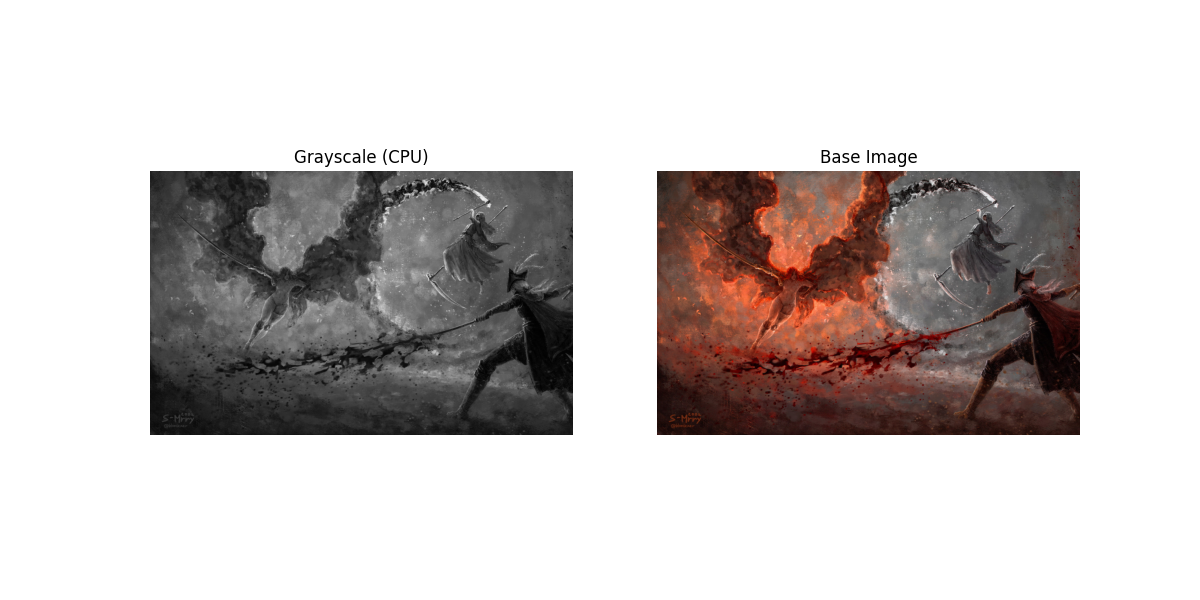
\includegraphics[scale=0.5]{src/grayscale_cpu.png}


\section{GPU greyscale}
We first import an image, then for convert it to grayscale with CUDA gpu

We resize the image then with the grayscale kernel 
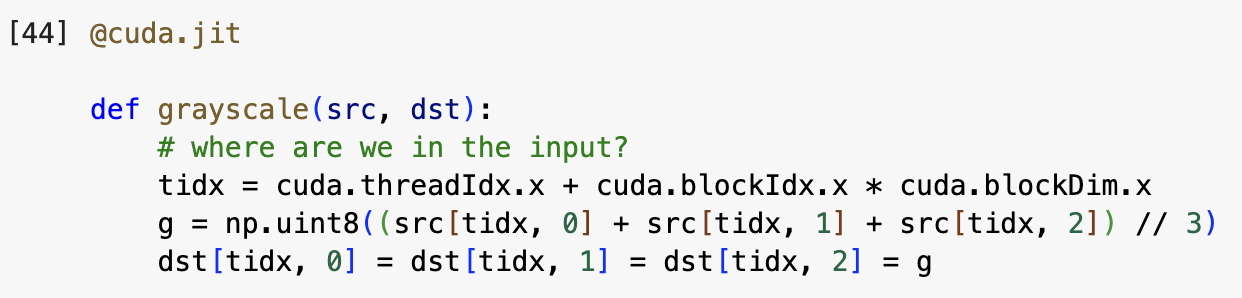
\includegraphics[scale=0.5]{src/grayscale.png}

we can now convert it to grayscale using the GPU and display it, so we see it's working and very faster than the CPU one
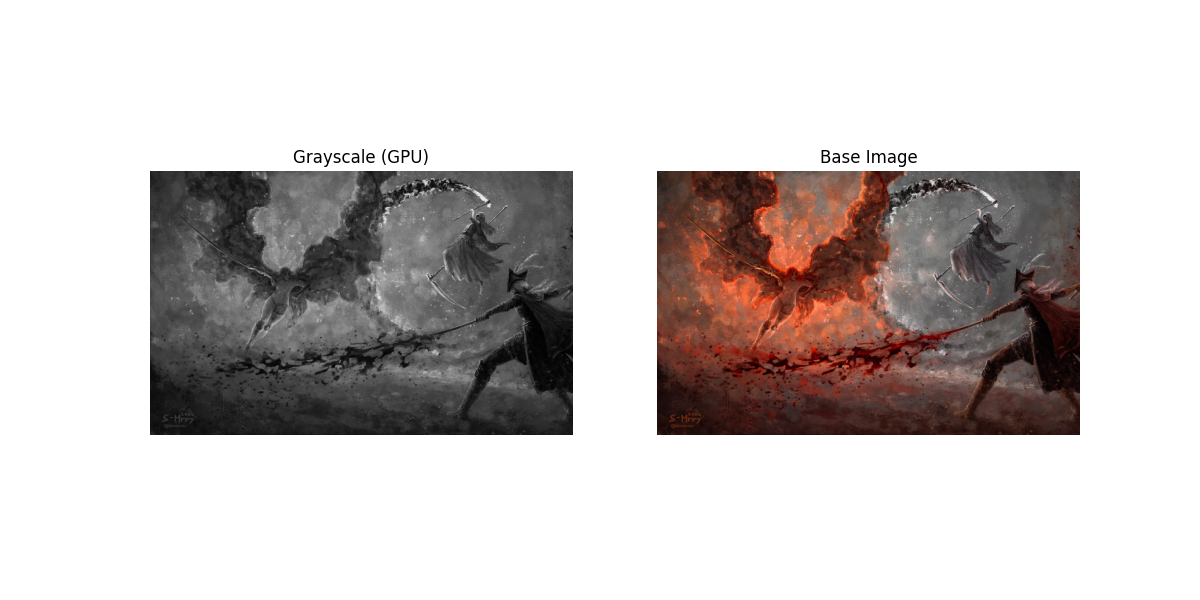
\includegraphics[scale=0.5]{src/grayscale_gpu.png}

\section{GPU block size comparaison}

We now try different block size to compare the execution time with GPU and block size

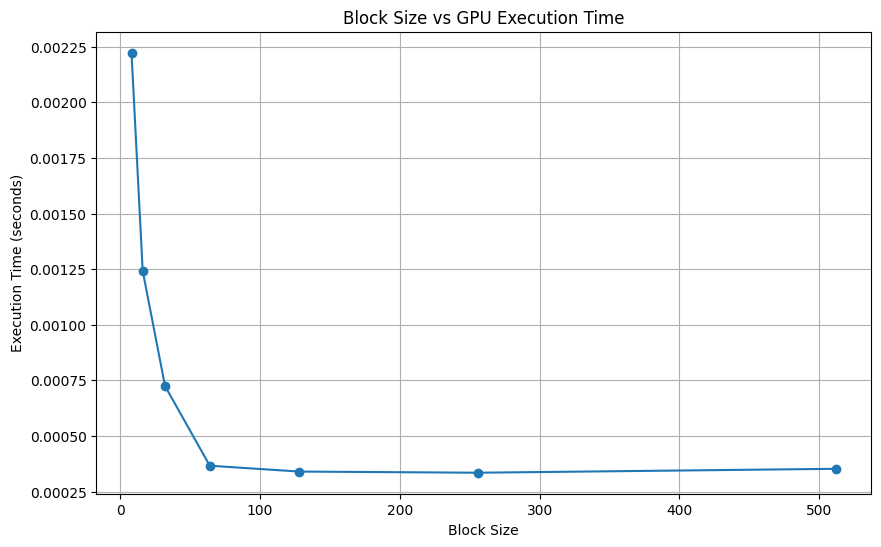
\includegraphics[scale=0.5]{src/block_size.png}

We can see that the execution time converges rapidly to 0.00035s, 
so we can deduce that it's not necessarily useful to set too large a block size

\end{document}
